%To compile as handout, use
%pdflatex "\def\ishandout{1} \input{filename.tex}"
%Defaults to non-handout mode (with slide reveals)
\ifdefined\ishandout
  \documentclass[handout]{beamer}
\else
  \documentclass{beamer}
\fi
 
\usepackage{econ103slides} 

\date{Lecture \# 9}
\begin{document} 

%%%%%%%%%%%%%%%%%%%%%%%%%%%%%%%%%%%%%%%%

\begin{frame}[plain]
	\titlepage 
	

\end{frame} 

%%%%%%%%%%%%%%%%%%%%%%%%%%%%%%%%%%%%%%%%

\begin{frame}
\centering \Huge Discrete RVs -- Part II

\end{frame}



%%%%%%%%%%%%%%%%%%%%%%%%%%%%%%%%%%%%%%%%

\begin{frame}
\frametitle{Linearity of Expectation}
\framesubtitle{Holds for Continuous RVs as well, but proof is different.}
Let $X$ be a RV and $a,b$ be constants. Then:
	$$E[a + bX] = a + bE[X]$$
\vspace{2em}
\begin{alertblock}{This is one of the most important facts in the course: the special case in which $E[g(X)] = g(E[X])$ is $g = a+bX$.}
\end{alertblock}
\end{frame}
%%%%%%%%%%%%%%%%%%%%%%%%%%%%%%%%%%%%%%%%
\begin{frame}
\frametitle{Example: Linearity of Expectation \hfill 
\includegraphics[scale = 0.05]{./images/clicker} }
Let $X \sim \mbox{Bernoulli}(1/3)$ and define $Y = 3X + 2$
\vspace{1em}

\begin{enumerate}
  \item What is $E[X]$? \pause \hspace{2em} \alert{$E[X] = 0 \times 2/3 + 1 \times 1/3 = 1/3$} \pause
  \item What is $E[Y]$? \pause \hspace{2em} \alert{$E[Y] = E[3X + 2] = 3E[X] + 2 = 3$}
\end{enumerate}
\end{frame}
%%%%%%%%%%%%%%%%%%%%%%%%%%%%%%%%%%%%%%%%

\begin{frame}
\frametitle{Proof: Linearity of Expectation For Discrete RV}

\begin{eqnarray*}
	E[a + bX] &=& \sum_{\mbox{all } x}  (a + bx) p(x)\\ \\
	 &=&  \sum_{\mbox{all } x} p(x) \cdot a + \sum_{\mbox{all } x}p(x) \cdot bx\\ \\
	&=&  a\sum_{\mbox{all } x} p(x) + b\sum_{\mbox{all } x} x \cdot p(x) \\ \\
	&=&  a + b E[X]
\end{eqnarray*}


\end{frame}
%%%%%%%%%%%%%%%%%%%%%%%%%%%%%%%%%%%%%%%%

\begin{frame}
\frametitle{Variance and Standard Deviation of a RV}
\framesubtitle{The Defs are the same for continuous RVs, but the method of calculating will differ.}

\begin{block}{Variance (Var)}
	$$\sigma^2 = Var(X) = E\left[ (X - \mu)^2\right] = E\left[ (X - E[X])^2\right]$$
\end{block}


\begin{block}{Standard Deviation (SD)}
$$\sigma = \sqrt{\sigma^2} = SD(X)$$
\end{block}


\end{frame}
%%%%%%%%%%%%%%%%%%%%%%%%%%%%%%%%%%%%%%%%
\begin{frame}
\frametitle{Key Point}

\alert{Variance and std.\ dev.\ are \emph{expectations of functions of a RV}} 

\vspace{1em}

It follows that: 
\begin{enumerate}
\item Variance and SD are constants
\item To derive facts about them you can use the facts you know about expected value
\end{enumerate}
\end{frame}
%%%%%%%%%%%%%%%%%%%%%%%%%%%%%%%%%%%%%%%%
\begin{frame}
\frametitle{How To Calculate Variance for Discrete RV?}
\framesubtitle{Remember: it's just a function of $X$!}


Recall that	$\displaystyle \mu = E[X] = \sum_{\mbox{all } x} xp(x)$


\vspace{3em}

$$Var(X) = E\left[ (X - \mu)^2 \right] =\sum_{\mbox{all } x} (x - \mu)^2 p(x)$$


\end{frame}
%%%%%%%%%%%%%%%%%%%%%%%%%%%%%%%%%%%%%%%%
\begin{frame}
\frametitle{Shortcut Formula For Variance}

This is \emph{not} the definition, it's a shortcut for doing calculations:
\begin{eqnarray*}
	Var(X) = E\left[ (X - \mu)^2 \right] = E[X^2] - \left(E[X]\right)^2
\end{eqnarray*}

\alert{We'll prove this in an upcoming lecture.}

\end{frame}

%%%%%%%%%%%%%%%%%%%%%%%%%%%%%%%%%%%%%%%%
\begin{frame}
\frametitle{Example: The Shortcut Formula \hfill 
\includegraphics[scale = 0.05]{./images/clicker}}
Let $X\sim \mbox{Bernoulli}(1/2)$.
\begin{enumerate}
  \item What is $E[X]$? \hspace{1em} \pause \alert{$E[X] = 0 \times 1/2 + 1 \times 1/2 = 1/2$} \pause
    \item What is $E[X^2]$? \pause \hspace{1em} \alert{$E[X^2] = 0^2 \times 1/2 + 1^2 \times 1/2 = 1/2$} \pause
    \item What is $Var(X)$? \pause \hspace{1em} \alert{$E[X^2] - \left( E[X] \right)^2 = 1/2 - (1/2)^2 = 1/4$} 
\end{enumerate}
\end{frame}
%%%%%%%%%%%%%%%%%%%%%%%%%%%%%%%%%%%%%%%%


\begin{frame}
\frametitle{Variance of Bernoulli RV -- via the Shortcut Formula}

\begin{block}{Step 1 -- $E[X]$} 
$\mu = E[X] = \displaystyle \sum_{x \in \{0,1\}} p(x) \cdot x = (1-p) \cdot 0 + p \cdot 1 = p$
\end{block}


\begin{block}{Step 2 -- $E[X^2]$} 
\begin{eqnarray*}
	E[X^2] = \sum_{x \in \{0,1\}} x^2 p(x) = 0^2 (1-p) + 1^2 p = p
\end{eqnarray*}
\end{block}


\begin{block}{Step 3 -- Combine with Shortcut Formula} 
\begin{eqnarray*}
	\sigma^2 = Var[X] = E[X^2] - \left(E[X]\right)^2 = \ p - p^2 =  p(1-p)
\end{eqnarray*}
\end{block}


\end{frame}
%%%%%%%%%%%%%%%%%%%%%%%%%%%%%%%%%%%%%%%%



\begin{frame}
\frametitle{Variance of Bernoulli RV -- Without Shortcut}

\alert{You will fill in the missing steps on Problem Set 5.}

\begin{eqnarray*}
	\sigma^2 &=& Var(X) = \sum_{x \in \{0,1\}} (x - \mu)^2 p(x)\\
	 &=& \sum_{x \in \{0,1\}} (x - p)^2 p(x)\\
	 &\vdots &\\ 
	 &=&p(1-p)
\end{eqnarray*}

%%%%%%%%%%%%%%%%%%%%%%%%%%%%%%%%%%%%%%%%


\end{frame}

\begin{frame}
\frametitle{Variance of a Linear Function  \hfill 
\includegraphics[scale = 0.05]{./images/clicker} }
Suppose $X$ is a random variable with $Var(X) = \sigma^2$ and $a,b$ are constants. What is $Var(a + bX)$? 
\begin{enumerate}[(a)]
	\item $\sigma^2$
	\item $a + \sigma^2$
	\item $b \sigma^2$
	\item $a + b \sigma^2$
	\item $b^2 \sigma^2$
\end{enumerate}

\end{frame}
%%%%%%%%%%%%%%%%%%%%%%%%%%%%%%%%%%%%%%%%
\begin{frame}
	\frametitle{Variance and SD are \emph{NOT} Linear}

\begin{eqnarray*}
Var(a + bX) &= &b^2 \sigma^2 \\\\
	SD(a + bX)&=& |b| \sigma
\end{eqnarray*}

\vspace{2em}
\begin{block}{These should look familiar from the related results for sample variance and std.\ dev. that you worked out on an earlier problem set.}

\end{block}

\end{frame}
%%%%%%%%%%%%%%%%%%%%%%%%%%%%%%%%%%%%%%%%
\begin{frame}
\frametitle{Variance of a Linear Transformation}

\begin{eqnarray*}
 Var(a + bX) &=& E\left[\left\{(a+bX) - E(a+bX)\right\}^2 \right] \\ 
 	&=& E\left[\left\{(a+bX) - (a+bE[X])\right\}^2 \right] \\
 	&=&E\left[\left(bX - bE[X]\right)^2 \right] \\ 
 	&=&E[b^2 (X - E[X])^2]\\ 
 	&=& b^2 E[(X-E[X])^2]\\ 
 	&=& b^2 Var(X) = b^2 \sigma^2
\end{eqnarray*}
\alert{The key point here is that variance is defined in terms of expectation and expectation is linear.}

\end{frame}
%%%%%%%%%%%%%%%%%%%%%%%%%%%%%%%%%%%%%%%%
\begin{frame}
	\begin{center}
		\Huge Binomial Random Variable	\\
		\large What we get if we sum a bunch of indep.\ Bernoulli RVs
	\end{center}
\end{frame}

%%%%%%%%%%%%%%%%%%%%%%%%%%%%%%%%%%%%%%%%

\begin{frame}
\frametitle{Binomial Random Variable}
Let $X = $ the sum of $n$ independent Bernoulli trials, each with probability of success $p$.  \alert{Then we say that:
		$X \sim \mbox{Binomial}(n,p)$} 

\vspace{2em}
\begin{block}{Parameters}
$p =$ probability of ``success,'' $n=$ \# of trials
\end{block}
\begin{block}{Support} 
$\{0, 1, 2, \hdots, n\}$ 
\end{block}
\begin{block}{Probability Mass Function (pmf)} 
$$p(x) = {n \choose x} p^x (1-p)^{n-x}$$ 
\end{block}
\end{frame}
%%%%%%%%%%%%%%%%%%%%%%%%%%%%%%%%%%%%%%%%

\begin{frame}
	\frametitle{\href{https://fditraglia.shinyapps.io/binom_cdf/}{http://fditraglia.shinyapps.io/binom\_cdf/}}
\framesubtitle{Try playing around with all three sliders. If you set the second to 1 you get a Bernoulli.}

\begin{figure}
	\fbox{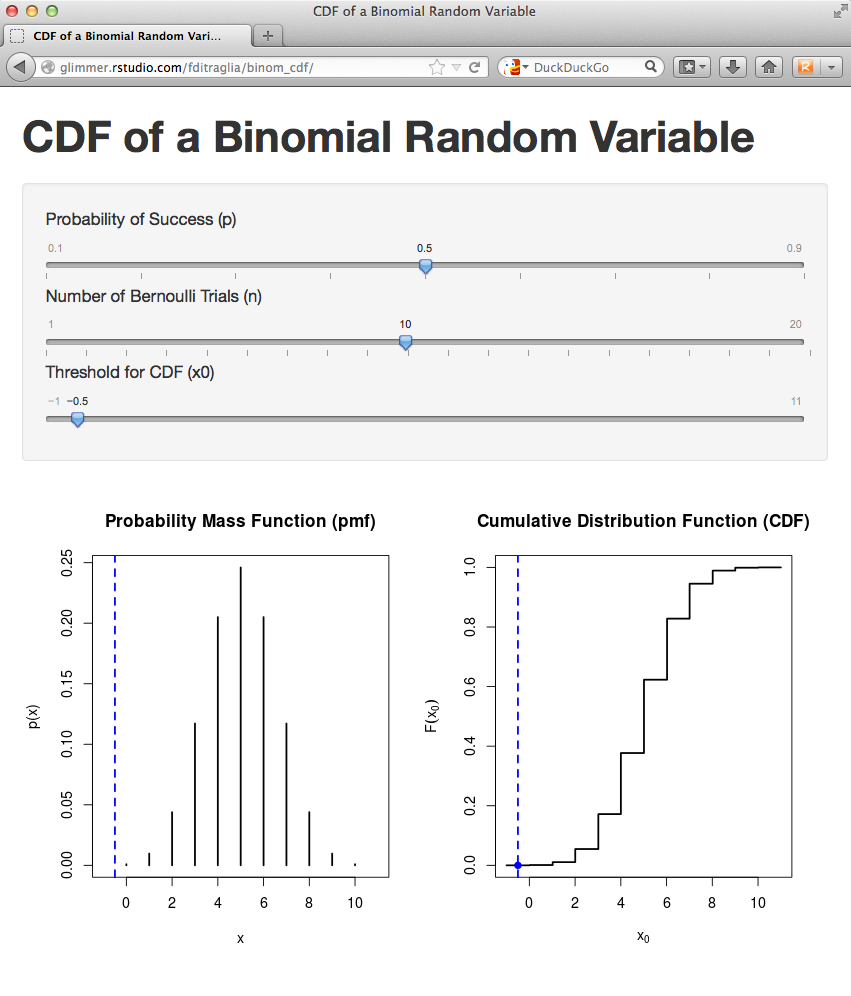
\includegraphics[scale = 0.2]{./images/binom_cdf_screenshot2}}
\end{figure}

\end{frame}

%%%%%%%%%%%%%%%%%%%%%%%%%%%%%%%%%%%%%%%%


\begin{frame}
	\frametitle{\href{http://fditraglia.github.com/Econ103Public/Rtutorials/Bernoulli_Binomial.html}{\small http://fditraglia.github.com/Econ103Public/Rtutorials/Bernoulli\_Binomial.html}}

\framesubtitle{Source Code on my \href{https://github.com/fditraglia/Econ103Public/blob/master/Rtutorials/Bernoulli_Binomial.R}{\fbox{Github Page}}}



\begin{figure}
	\fbox{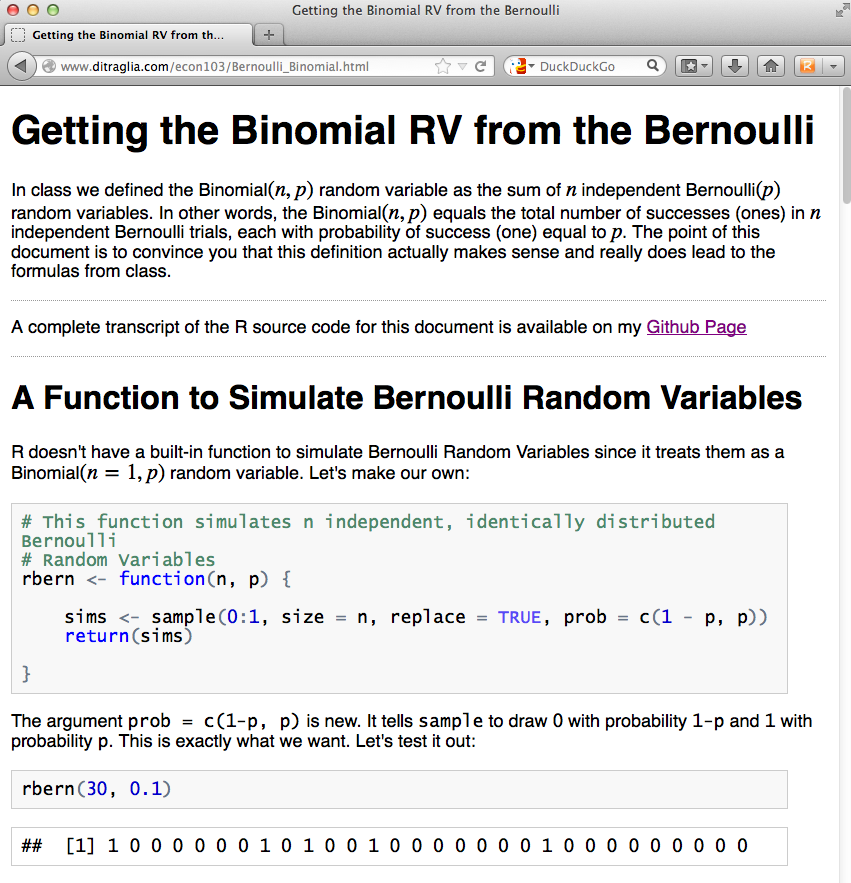
\includegraphics[scale = 0.15]{./images/binom_bernoulli_sim_screenshot}}
\end{figure}

\begin{alertblock}{Don't forget this!}
 Binomial RV counts up the \emph{total} number of successes (ones) in $n$ indep.\ Bernoulli trials, each with prob.\ of success $p$.
\end{alertblock}

\end{frame}

%%%%%%%%%%%%%%%%%%%%%%%%%%%%%%%%%%%%%%%%

\begin{frame}
\frametitle{Where does the Binomial pmf come from? 
\includegraphics[scale = 0.05]{./images/clicker} }
\begin{block}{Question}
Suppose we flip a fair coin 3 times. What is the probability that we get exactly 2 heads?
\end{block}

\pause

\begin{block}{Answer}
Three basic outcomes make up this event: $\{HHT, HTH, THH\}$, each has probability $1/8 = 1/2 \times 1/2 \times 1/2$. Basic outcomes are mutually exclusive, so sum to get \alert{$3/8 = 0.375$}
\end{block}

\end{frame}
%%%%%%%%%%%%%%%%%%%%%%%%%%%%%%%%%%%%%%%%
\begin{frame}
\frametitle{Where does the Binomial pmf come from?}
\begin{block}{Question}
Suppose we flip an \emph{unfair} coin 3 times, where the probability of heads is 1/3. What is the probability that we get exactly 2 heads?
\end{block}



\begin{block}{Answer}
  No longer true that \emph{all} basic outcomes are equally likely, but those with exactly two heads \emph{\alert{still are}} 
	\begin{eqnarray*}
	 P(HHT) &=&  (1/3)^2 (1 - 1/3) =  2/27\\ 
	 P(THH) &=&2/27\\ 
	 P(HTH) &=&2/27 
	\end{eqnarray*}
	Summing gives \alert{$2/9 \approx 0.22$}
\end{block}
\end{frame}
%%%%%%%%%%%%%%%%%%%%%%%%%%%%%%%%%%%%%%%%
\begin{frame}
  \frametitle{Where does the Binomial pmf come from?}
\framesubtitle{Starting to see a pattern?}

Suppose we flip an unfair coin \emph{4} times, where the probability of heads is 1/3. What is the probability that we get exactly 2 heads?

\vspace{2em}



\begin{columns}
\column{0.35\textwidth}
\begin{tabular}{cc}
HHTT&TTHH\\
HTHT&THTH\\
HTTH&THHT
\end{tabular}

\column{0.55\textwidth}
\alert{Six equally likely, mutually exclusive basic outcomes make up this event:}
$${4\choose 2}(1/3)^2(2/3)^2$$
\end{columns}

\end{frame}

%%%%%%%%%%%%%%%%%%%%%%%%%%%%%%%%%%%%%%%%

\begin{frame}
  \frametitle{Multiple RVs \emph{at once} - Definition of Joint PMF}
Let $X$ and $Y$ be discrete random variables. The joint probability mass function $p_{XY}(x,y)$ gives the probability of each pair of realizations $(x,y)$ in the support:
\Large
 $$\boxed{p_{XY}(x,y) = P(X = x \cap Y=y)}$$

\end{frame}
%%%%%%%%%%%%%%%%%%%%%%%%%%%%%%%%%%%%%%%%
\begin{frame}
\frametitle{Example: Joint PMF in Tabular Form}

\begin{table}
\begin{tabular}{|cc|ccc|}
\hline
&&\multicolumn{3}{c|}{$Y$}\\
&&1 & 2&3\\
\hline
\multirow{4}{*}{$X$}
&0& \multicolumn{1}{|c}{\alert{1/8}} & \alert{0}& \alert{0}\\
&1& \multicolumn{1}{|c}{\alert{0}} & \alert{1/4}&\alert{1/8}\\
&2& \multicolumn{1}{|c}{\alert{0}} & \alert{1/4}&\alert{1/8}\\
&3& \multicolumn{1}{|c}{\alert{1/8}} & \alert{0}&\alert{0}\\
\hline
\end{tabular}
\end{table}

\end{frame}
%%%%%%%%%%%%%%%%%%%%%%%%%%%%%%%%%%%%%%%%
\begin{frame}
\frametitle{Plot of Joint PMF}
\begin{figure}
	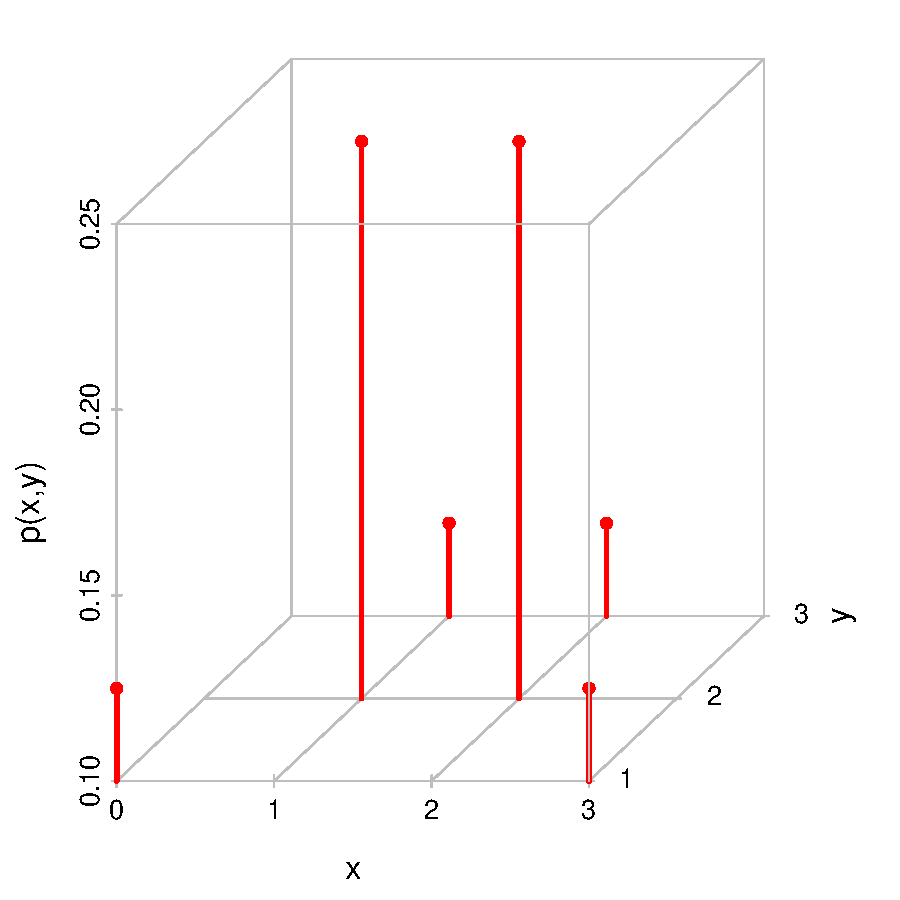
\includegraphics[scale = 0.53]{./images/joint_dist}
\end{figure}

\end{frame}



%%%%%%%%%%%%%%%%%%%%%%%%%%%%%%%%%%%%%%%%
\begin{frame}
\frametitle{What is $p_{XY}(1,2)$? \hfill 
\includegraphics[scale = 0.05]{./images/clicker}}

\begin{table}
\begin{tabular}{|cc|ccc|}
\hline
&&\multicolumn{3}{c|}{$Y$}\\
&&1 & 2&3\\
\hline
\multirow{4}{*}{$X$}
&0& \multicolumn{1}{|c}{\alert{1/8}} & \alert{0}& \alert{0}\\
&1& \multicolumn{1}{|c}{\alert{0}} & \alert{1/4}&\alert{1/8}\\
&2& \multicolumn{1}{|c}{\alert{0}} & \alert{1/4}&\alert{1/8}\\
&3& \multicolumn{1}{|c}{\alert{1/8}} & \alert{0}&\alert{0}\\
\hline
\end{tabular}
\end{table}

\pause



$$p_{XY}(1,2) =   P(X=1 \cap Y =2) =  \alert{1/4}$$

\end{frame}

%%%%%%%%%%%%%%%%%%%%%%%%%%%%%%%%%%%%%%%%
\begin{frame}
\frametitle{What is $p_{XY}(2,1)$? \hfill 
\includegraphics[scale = 0.05]{./images/clicker}}

\begin{table}
\begin{tabular}{|cc|ccc|}
\hline
&&\multicolumn{3}{c|}{$Y$}\\
&&1 & 2&3\\
\hline
\multirow{4}{*}{$X$}
&0& \multicolumn{1}{|c}{\alert{1/8}} & \alert{0}& \alert{0}\\
&1& \multicolumn{1}{|c}{\alert{0}} & \alert{1/4}&\alert{1/8}\\
&2& \multicolumn{1}{|c}{\alert{0}} & \alert{1/4}&\alert{1/8}\\
&3& \multicolumn{1}{|c}{\alert{1/8}} & \alert{0}&\alert{0}\\
\hline
\end{tabular}
\end{table}

\pause

$$p_{XY}(2,1) =  P(X=2 \cap Y =1) = \alert{0}$$

\end{frame}

%%%%%%%%%%%%%%%%%%%%%%%%%%%%%%%%%%%%%%%%

\begin{frame}
\frametitle{Properties of Joint PMF}
	\begin{enumerate}
		\item $0\leq p_{XY}(x,y)\leq 1$ for any pair $(x,y)$
		\item The sum of $p_{XY}(x,y)$ over all pairs $(x,y)$ in the support is 1:
			$$\sum_{x}\sum_{y} p(x,y) = 1$$
	\end{enumerate}
\end{frame}


%%%%%%%%%%%%%%%%%%%%%%%%%%%%%%%%%%%%%%%%
\begin{frame}
\frametitle{Does this satisfy the properties of a joint pmf? \hfill 
\includegraphics[scale = 0.05]{./images/clicker}}
\alert{(A = YES, B = NO)}
\begin{table}
\begin{tabular}{|cc|ccc|}
\hline
&&\multicolumn{3}{c|}{$Y$}\\
&&1 & 2&3\\
\hline
\multirow{4}{*}{$X$}
&0& \multicolumn{1}{|c}{\alert{1/8}} & \alert{0}& \alert{0}\\
&1& \multicolumn{1}{|c}{\alert{0}} & \alert{1/4}&\alert{1/8}\\
&2& \multicolumn{1}{|c}{\alert{0}} & \alert{1/4}&\alert{1/8}\\
&3& \multicolumn{1}{|c}{\alert{1/8}} & \alert{0}&\alert{0}\\
\hline
\end{tabular}
\end{table}

\pause

\begin{enumerate}
	\item $p(x,y) \geq 0$ for all pairs $(x,y)$
	\item $\sum_x\sum_{y} p(x,y) = 1/8 + 1/4 + 1/8 + 1/4 + 1/8 + 1/8 = 1$
\end{enumerate}

\end{frame}

%%%%%%%%%%%%%%%%%%%%%%%%%%%%%%%%%%%%%%%%
\begin{frame}
\frametitle{Joint versus Marginal PMFs}

\begin{block}{Joint PMF}
 $p_{XY}(x,y) = P(X=x \cap Y=y)$
\end{block}



\begin{block}{Marginal PMFs}
$p_X(x) = P(X=x)$\\ $p_Y(y) = P(Y=y)$
\end{block}



\vspace{1em}

\alert{You can't calculate a joint pmf from marginals alone but you \emph{can} calculate marginals from the joint!}

\end{frame}
%%%%%%%%%%%%%%%%%%%%%%%%%%%%%%%%%%%%%%%%
\begin{frame}
\frametitle{Marginals from Joint}

	$$\boxed{p_X(x) = \sum_{\mbox{all } y} p_{XY}(x,y)}$$
	
	$$\boxed{p_Y(y) = \sum_{\mbox{all } x} p_{XY}(x,y)}$$


\begin{block}{Why?}
	\begin{eqnarray*}
	p_Y(y) &=& P(Y=y) = P\left( \bigcup_{\mbox{all } x}\left\{ X=x \cap Y=y \right\}  \right)\\
		&=& \sum_{\mbox{all } x} P(X=x \cap Y=y) = \sum_{\mbox{all } x} p_{XY}(x,y)
	\end{eqnarray*}
\end{block}
\end{frame}
%%%%%%%%%%%%%%%%%%%%%%%%%%%%%%%%%%%%%%%%
\begin{frame}
\frametitle{To get the marginals sum ``into the margins'' of the table.}

\begin{table}
\begin{tabular}{|cc|ccc|c|}
\hline
&&\multicolumn{3}{c|}{$Y$}&\\
&&1 & 2&3&\\
\hline
\multirow{4}{*}{$X$}
&0& \multicolumn{1}{|c}{\alert{1/8}} & \alert{0}& \alert{0}&\onslide<2->{\textcolor{blue}{1/8}}\\
&1& \multicolumn{1}{|c}{\alert{0}} & \alert{1/4}&\alert{1/8}&\onslide<3->{\textcolor{blue}{3/8}}\\
&2& \multicolumn{1}{|c}{\alert{0}} & \alert{1/4}&\alert{1/8}&\onslide<4->{\textcolor{blue}{3/8}}\\
&3& \multicolumn{1}{|c}{\alert{1/8}} & \alert{0}&\alert{0}&\onslide<5->{\textcolor{blue}{1/8}}\\
\hline 
&&&&&\onslide<5->{\textcolor{blue}{1}}\\
\hline
\end{tabular}
\end{table}

\begin{eqnarray*}
	\onslide<2->{p_X(0) &=& 1/8 + 0 + 0 = 1/8}\\
	\onslide<3->{p_X(1) &=&0 + 1/4 + 1/8 = 3/8}\\
	\onslide<4->{p_X(2) &=&0 + 1/4 + 1/8 = 3/8}\\
	\onslide<5->{p_X(3) &=&1/8 + 0 + 0 = 1/8}
\end{eqnarray*}


\end{frame}

%%%%%%%%%%%%%%%%%%%%%%%%%%%%%%%%%%%%%%%%

\begin{frame}
\frametitle{What is $p_Y(2)$? \hfill 
\includegraphics[scale = 0.05]{./images/clicker}}

\begin{table}
\begin{tabular}{|cc|ccc|c|}
\hline
&&\multicolumn{3}{c|}{$Y$}&\\
&&1 & 2&3&\\
\hline
\multirow{4}{*}{$X$}
&0& \multicolumn{1}{|c}{\alert{1/8}} & \alert{0}& \alert{0}&\\
&1& \multicolumn{1}{|c}{\alert{0}} & \alert{1/4}&\alert{1/8}&\\
&2& \multicolumn{1}{|c}{\alert{0}} & \alert{1/4}&\alert{1/8}&\\
&3& \multicolumn{1}{|c}{\alert{1/8}} & \alert{0}&\alert{0}&\\
\hline 
&&\onslide<2->{\textcolor{blue}{1/4}}&\onslide<3->{ \textcolor{blue}{1/2} }& \onslide<4->{\textcolor{blue}{1/4}} &\onslide<4->{\textcolor{blue}{1}}\\
\hline
\end{tabular}
\end{table}

\begin{eqnarray*}
	\onslide<2->{p_Y(1) &=& 1/8 + 0 + 0 + 1/8 = 1/4}\\
	\onslide<3->{p_Y(2) &=&0 + 1/4 + 1/4 + 0 = 1/2}\\
	\onslide<4->{p_Y(3) &=&0 + 1/8 + 1/8 + 0= 1/4}
\end{eqnarray*}


\end{frame}


\end{document}
